\chapter{Conteo de Cruces}
Dentro del problema que tenemos que resolver, un aspecto fundamental es el conteo de cruces, tanto la soluci�n exacta,
como las heuristicas necesitan saber muchas veces (ya sea durante la etapa de construcci�n, como para decidir si cierto cambio genera un dibujo mejor) cuantos cruces hay en el dibujo. Por esta raz�n consideramos que un aspecto importante a optimizar para lograr mejorar el desempe�o de nuestros algoritmos es precisamente el conteo de cruces.

Lo primero que se puede observar es que los cruces en el dibujo depende solamente de la posici�n relativa de los nodos en las particiones. Se produce un cruce si hay dos nodos en una partici�n $v_i$, $v_j$ que estan relacionados con un $w_k$ y $w_p$ tal que $v_i$ esta $``arriba''$ de $v_j$ y $w_k$ esta $``abajo''$ de $w_p$.

Podemos entonces caracterizar en que casos se producen cruces:
Dado un orden de los nodos $p_1=<v_1,v_2,...,v_n>$ en una partici�n y un orden $p_2=<w_1,w_2,...,w_q>$ en la otra partici�n , se produce un cruce si existen ejes $(v_i,w_j)$, $(v_k,w_p)$ tal que $i<k \wedge p<j$.

De esta manera un primer algoritmo para contar los cruces, consiste en tomar cada par de ejes y comparar las posiciones relativas de sus nodos. Hacer esto tiene un costo $\theta(m^2)$, siendo $m$ la cantidad de ejes, ya que la cantidad de posibles pares de ejes es $\binom{m}{2} = \frac{m*(m-1)}{2}$. Este costo puede ser excesivo, principalmente en grafos densos, donde m puede ser del orden de $n_1*n_2$, siendo $n_i$ la cantidad de nodos en las particion i.

Buscamos entonces alg�n algoritmo que nos de un orden mejor que $O(m^2)$. 

Si se ordenan los ejes del grafo primero por su componente en la particion $p_1$ y luego por su componente $p_2$, es decir si $e_i=(i_1,i_2)$ y $e_j=(j_1,j_2)$ son ejes del grafo, consideramos que $e_i < e_j \Leftrightarrow i_1 < j_1 \vee (i_1 == j_1 \wedge i_2 < j_2)$ y consideramos luego el orden en el que quedan las segundas componentes, podemos ver que cada inversi'on es un cruce. Una inversi�n en el orden $\pi=<a_1,a_2,....a_n>$ es un par $\{a_i,a_j\}$ tal que $a_i > a_j$ $\wedge$ $i<j$. Esto es asi porque como primero se ordena por la primer componente (en verdad es la componente de la primer partici�n, pero para simplificar la notaci�n nos referiremos a dicha componente como la primer componente) y luego por la segunda, si hay una inversion es porque para los ejes $\{v_k,a_i\}$ y $\{v_p,a_j\}$ val�a que $v_k < v_p \wedge a_i > a_j$, y esa es la condici�n para que se produzca un cruce.

%TODO: ver si no hay q explicar mejor como se puede calcular eso
Entonces si ordenamos los ejes de esa manera y despu�s contamos las inversiones, podemos obtener el numero de cruces. Para ordenar a los ejes se puede utilizar radix sort (suponiendo que los ejes tienen como componentes las posiciones relativas de los ejes (o que estas se pueden obtener facilmente), lo cual se puede calcular en caso de que esa informaci�n no este disponible con un costo de $n_1 + n_2 + m $, con $n_i$ la cantidad de nodos de la partici'on i) y luego considerar el arreglo que tiene a las segundas componentes de los ejes como elementos, aplicar insertion sort y por cada cambio de posici�n que se hace para un elemento, contar una inversi�n y por lo tanto un cruce. Esto �ltimo tendr�a un costo $O(m+c)$, con c la cantidad de cruces. En el peor caso, todos los ejes se cruzan por lo que tendr�amos un costo $O(m^2)$ nuevamente.

Veamos un ejemplo de como funciona este algoritmo:
Consideremos el siguiente grafo bipartito:
\begin{figure}[H]
    \centering
     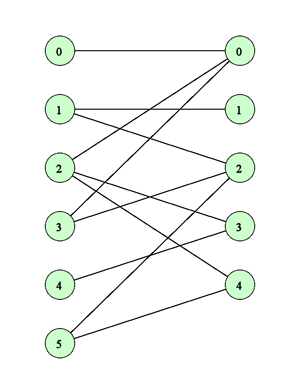
\includegraphics[scale=0.8]{./figuras/cruces/ejemplo1.png}
     \caption{Grafo de ejemplo para la aplicacion de los algoritmos de conteo de cruces}
     \label{ejemplo1}
\end{figure} 

Ahora ordenamos los ejes de acuerdo a su primer componente y luego a su segunda, obtenemos lo siguiente:

$$\left\langle (0,0),(1,1),(1,2),(2,0),(2,3),(2,4),(3,0),(3,2),(4,3),(5,2),(5,4)\right\rangle$$

Entonces el arreglo formado por las segundas componentes es el siguiente:

$$\left\langle0,1,2,\textcolor{Red}{0},3,4,0,2,3,2,4\right\rangle$$

Entonces, aplicamos selection sort. El 0 (de color rojo),recorre dos posiciones antes de insertarse en su posici�n correcta.

$$\left\langle0,0,1,2,3,4,\textcolor{Red}{0},2,3,2,4\right\rangle$$

Luego el tercer 0 se swapea cuatro veces:
 
$$\left\langle0,0,0,1,2,3,4,\textcolor{Red}{2},3,2,4\right\rangle$$

El segundo 2 cambia dos veces de posici�n:

$$\left\langle0,0,0,1,2,2,3,4,\textcolor{Red}{3},2,4\right\rangle$$

Ahora el segundo 3 cambia una vez de posici�n:

$$\left\langle0,0,0,1,2,2,3,3,4,\textcolor{Red}{2},4\right\rangle$$

Finalmente el �ltimo 2 es swapeado tres posiciones.

Entonces la cantidad de cruces del grafo es: $2+4+2+1+3 = 12$

Si bien en el caso general este algoritmo tiene un mejor orden, en peor caso sigue siendo $O(m^2)$.

Veamos un tercer acercamiento al problema: Sea $\sharp v_2 =\left|v_2\right|$ la cantidad de nodos de la particion 2. Consideremos un arbol binario con $2^k$ hojas donde k es tal que $2^{k-1} < \sharp v_2 <= 2^{k}$ de modo de que cada nodo este en una hoja (podria haber hojas que no tengan a ningun nodo), dispuestos de izquierda a derecha seg�n su orden en la partici�n. Este �rbol tiene $2^{k+1}-1$ nodos. Ademas $k=\left\lceil log_2(\sharp v2)\right\rceil$

Lo que vamos a hacer es ordenar a los ejes como lo hicimos para el algoritmo anterior. Luego lo que haremos es agregar a los ejes segun dicho orden. Agregar el eje consiste en incrementar en uno el contador, en principio inicializado en 0, de la hoja correspondiente al nodo de la segunda componente del eje. Ademas se incrementa tambi�n en uno el contador del padre de dicha hoja y este incremento se va propagando hacia arriba.

Cada vez que insertamos un eje, en cada nivel, si estamos parado en un nodo izquierdo aumentamos el n�mero de cruces segun el valor del hermano del nodo.

El procedimiento puede resultar confuso en un principio por lo cual mostraremos un ejemplo de su aplicaci�n.
Apliquemos el algoritmo para el grafo de \ref{ejemplo1}:

Como tenemos $\sharp v_2 = 5$, el arbol va a tener 8 hojas y un total de 15 nodos.
 
\begin{figure}[H]
    \centering
     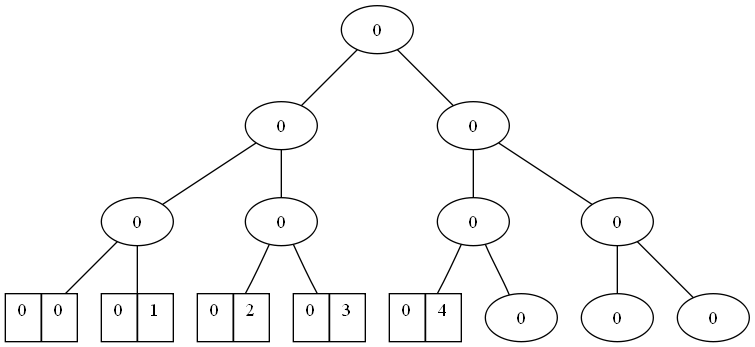
\includegraphics[scale=0.4]{./figuras/cruces/arbol.png}
     \caption{�rbol para contar cruces en el grafo de ejemplo}
     \label{arbol}
\end{figure} 

Los nodos cuadrados son las hojas que representan a un nodo (el nodo es el numero de la derecha). Cada nodo tiene un contador , en principio inicializado en 0. El contador de cruces tambi�n esta inicializado en 0.

Recordemos que luego de ordenar los ejes el vector era:
$$\left\langle(0,0),(1,1),(1,2),(2,0),(2,3),(2,4),(3,0),(3,2),(4,3),(5,2),(5,4)\right\rangle$$

Lo primero que hacemos entonces es insertar el eje (0,0), de modo que se incrementa el contador de la hoja 0 y este incremento se propaga hacia arriba. Como 0 esta en un nodo izquierdo, lo que se hace es sumar a la cantidad de cruces el valor del contador del hermano de 0 (la hoja 1). Esto porque, porq el valor de dicho contador indica la cantidad de ejes insertados que terminaban en 1, pero ademas dado el orden que se usa para agregar a los nodos, sabemos que la primer coordenada de estos ejes que terminaban en 1 era menor que la del ejes que estoy insertando ahora, por lo tanto hay un cruce.
Al subir de nivel, como tambi�n estamos en un nodo izquierdo, agregamos a la cantidad de cruces el valor del contador del hermano correspondiente. En este caso, dicho contador guarda la cantidad de ejes agregados que terminan en 2 0 3. Y asi sucesivamente.

Luego de esta inserci�n obtenemos el siguiente �rbol:
\begin{figure}[H]
    \centering
     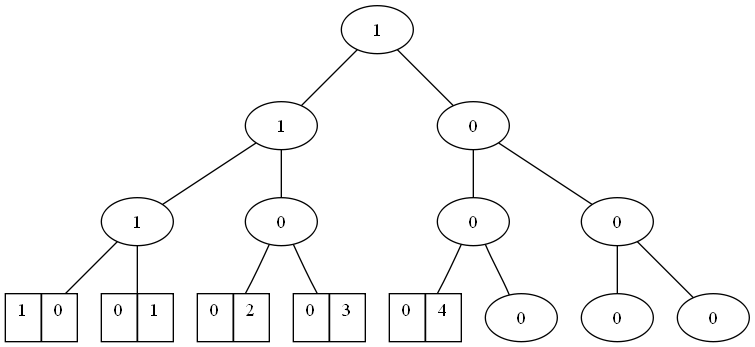
\includegraphics[scale=0.4]{./figuras/cruces/arbol2.png}
     \caption{�rbol con el eje (0,0) insertado}
     \label{arbol2}
\end{figure} 

De manera analoga, se insertan los ejes (1,1) y (1,2), sin que se generen cruces, en este caso el arbol queda de la siguiente manera:

\begin{figure}[H]
    \centering
     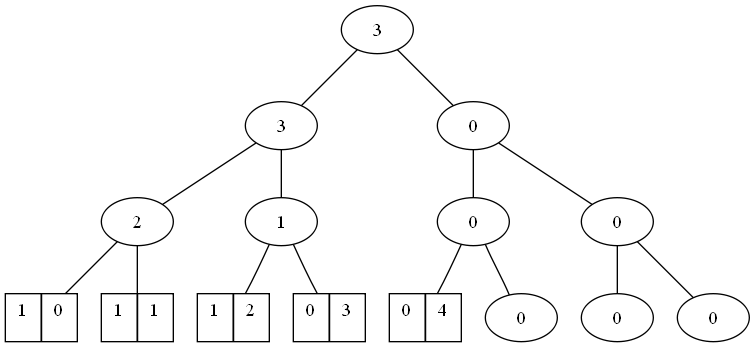
\includegraphics[scale=0.4]{./figuras/cruces/arbol3.png}
     \caption{�rbol con los ejes (0,0),(1,1) y (1,2) insertados}
     \label{arbol3}
\end{figure} 

Luego corresponde insertar el eje (2,0). Incrementamos en uno el contador de la hoja 0. Como es un nodo izquierdo, sumamos a cantidad de cruces el valor de la hoja 1, que es 1. Este incremento corresponde al cruce del eje (2,0) con el ejes (1,1). Subimos un nivel e incrementamos en 1 el contador del padre de la hoja 0. Nuevamente sumamos al contador de cruces, el valor del contador del hermano del nodo donde estamos parados, ya que otra vez estamos en un nodo izquierdo. Este nuevo incremento corresponde al cruce entre el eje (2,0) y el eje (1,2). Subimos por �ultimo hasta la raiz, incrementando el valor de los contadores y sumando el valor de los contadores de los nodos derechos siempre que caemos en nodo izquierdo. En particular en este caso, volvemos a caer en un nodo izquierdo, pero el contador de su hermano es 0. Esto se debe a que todavia no insertamos ning�n eje que terminara en 4.

\begin{figure}[H]
    \centering
     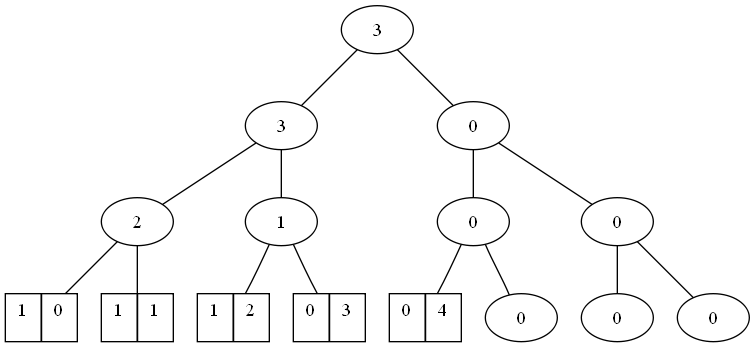
\includegraphics[scale=0.4]{./figuras/cruces/arbol3.png}
     \caption{�rbol con los ejes (0,0),(1,1),(1,2) y (2,0) insertados}
     \label{arbol3}
\end{figure} 


El procedimiento se repite hasta colocar todos los ejes.

Veamos que costo tiene este algoritmo: vamos a mirar todos los ejes. Para cada ejes recorremos el arbol desde una hoja hasta la raiz. Como el arbol tiene $2^k$ hojas, tiene $log_2(2^k)$ de altura, pero $log_2(2^k)=k=\left\lceil log_2(\sharp v2)\right\rceil$. Por lo tanto, el costo de insertar todos los ejes es $O(m*log(\sharp v_2) )$

Ahora bien, si en vez de ordenar primero por la primer componente y luego con respecto a la segunda, podriamos hacer el mismo procedimiento pero ordenando primero por la segunda, luego por la primera y armando el arbol para $v_1$. Entonces, en particular el procedimiento se podria realizar utilizando el  $v_i$ de menor cardinal. Con lo cual el costo de las inserciones es de $O(m*log(min_{i=1,2}(\sharp v_i) )$

Repasando tenemos 3 algoritmos para calcular los cruces:
\begin{itemize}
\item El primero, consiste en revisar todo par de ejes. Tiene un costo $O(m^2)$
\item El segundo ordena los ejes y luego realiza insertion sort para contar inversiones. Tiene un costo de $O(m+c)$
\item El tercero utiliza el arbol binario para contar inversiones. Tiene un orden $O(m+m*log(min_{i=1,2}(\sharp(v_i))))$
\end{itemize}

Todas estos algoritmos requieren conocer el ``orden'' de los nodos en cada particion, lo cual podria hacerse, en $O(\sharp(v_1) + \sharp(v_2))$ costo que se suma a los algoritmos en caso de que no se tenga dicha informaci�n.

Si $m > log(min_{i=1,2}(\sharp(v_i)))$ combiene utilizar el tercer algoritmo, pues tiene una complejidad menor que la de los otros dos.

Si en cambio $m < log(min_{i=1,2}(\sharp(v_i)))$ (un grafo con muy pocos ejes) resulta conveniente utilizar el segundo algoritmo ya que provee un mejor orden.







   
